\documentclass[12pt,a4paper]{article}
\usepackage{graphicx}
\usepackage[toc,page]{appendix}
\usepackage{xcolor}
\usepackage{listings}
\lstset{basicstyle=\ttfamily,
  showstringspaces=false,
  commentstyle=\color{red},
  keywordstyle=\color{blue}
}


\begin{document}
\begin{titlepage}
	\centering
	
\includegraphics[width=0.55\textwidth]{tentacle.png}\par\vspace{1cm}
	{\scshape\LARGE Smart Soft-Robotics Tentacle Documentation\par}
	\vspace{1cm}
	{\scshape\Large NoodleBot\par}
	\vspace{1.5cm}
	{\itshape \textbf{Byron Becker, Surjith Singh, Vidur Sarin, Adam Seifkas, Stan James, Ryan Riley}\par}
	{\large \today\par}
\end{titlepage}

\tableofcontents

\newpage
\section{Introduction}

The NoodleBot team is creating a robot tentacle from a pool noodle, para cord, stepper motors, a micro controller, and machine learning software. The device is intended for those with accessibility concerns and will allow those with a limited range of motion to reach out and potentially manipulate objects.

\section{Overview}

\begin{figure}[h]
\centering
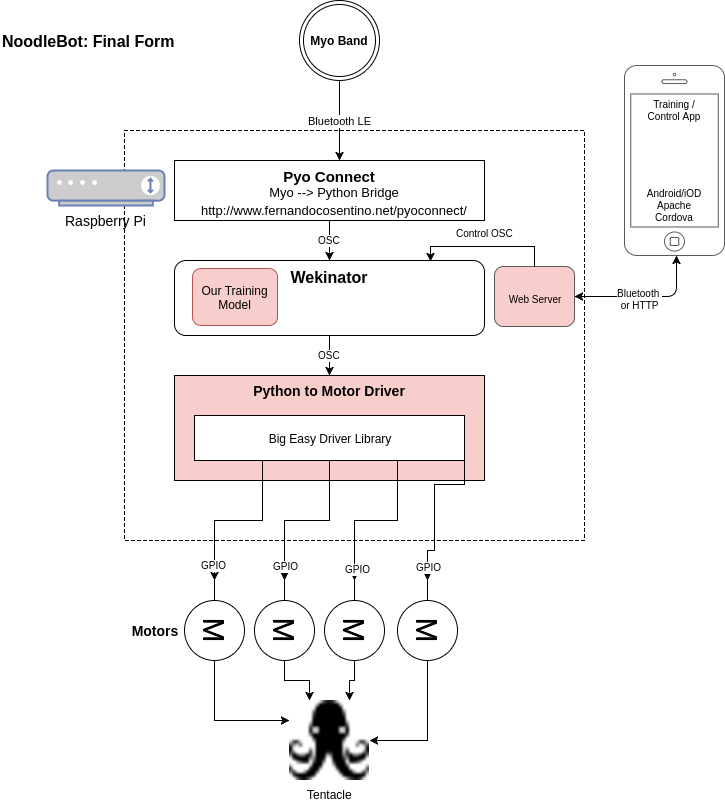
\includegraphics[width=0.75\textwidth]{SoftwareFlow.png}\par\vspace{1cm}
\caption{Software Flow}
\label{fig:flow}
\end{figure}


\section{Hardware}

Our first concern was creating the physical device

\section{Software}

\subsection{Myo Osc and Related Python Scripts}

\subsection{Mobile App}

\subsection{Machine Learning with Wekinator}

\subsection{Hardware Control Code}

\section{Challenges}

\section{Future Work}



\end{document}
